\section{Posisjonsmåler}
\label{sec:pos_måler}

\subsection{Teori}

% Enpolet målesignal
%   - Referanse til signaljord
% Signalkilde -[signal]-> signalmottaker / last
% Målevariabel -> Føler -> Omsetter -> Målesignal

% Standardiserte signalnivåer
% 1 - 5V
% Elevated Zero
%   - Muliggjør deteksjon av feil
%   - Vanskelig å måle 0, krever negativ strømforsyning
%   - Ledningsbrud
%   - Muliggjør alarmgrenser utenfor ordinært måleområde

Posisjonsmåling kan enten være en vinkelmåling eller en strekningsmåling. For en servomotor er målevariabelen vinkel nyttigst. Potensiometer kan brukes som en føler for måleveraibelen. Med en spennig over potensiometeret, vil dette generere et enpolet målesignal, med en spenningsforskjell til jord.

For å lettere detektere feil er standardiserte målesignaler med elevated zero nyttig. Ledningsbrudd blir da lettere å oppdage. I tillegg er det vanskelig å måle spenninger rundt $0V$, med laveste signal over $0V$ vil ikke dette bli et problem. Derfor er det lurt å omformere målesignalet til et standardisert målesignal.

\subsection{Metode}

\begin{figure}[h]
    \centering
    \begin{circuitikz}[scale=0.7, transform shape]
    \ctikzset{resistor = european}

    \draw (0, 0)
    to[short, o-, l=15<\volt>] ++(0, 0)
    to[R=12<\kilo\ohm>] ++(2, 0)
    to[potentiometer, n=R2] ++(0, -2)
    to[R=8.2<\kilo\ohm>] ++(-2, 0)
    to[short, -o, l=-15<\volt>] ++(0, 0);

    \draw[->] (R2) ++(-0.4, 0.3)
    -- ++(0, -0.6);
    
    \draw (R2) ++(0.2, 0.4)
    node[anchor=west]{\SI{5}{\kilo\ohm}};

    \draw (R2.wiper)
    to[short, -o] ++(0.5, 0)
    node[anchor=west]{$\theta$};
    
\end{circuitikz}
    \caption{Potensiometeret i motorkortet. Figur hentet fra \cite{AnalogMotorlabbOppgaver}}
    \label{fig:posisjon_maler_potmeter}
\end{figure}

\begin{table}[h]
    \centering
    \caption{Motstander og kondensatorer i posisjonomformer. Verdiene er hentet fra \cite{AnalogMotorlabbOppgaver}}
    \begin{tabular}{lll}
        \toprule
        Størrelse & Verdi & Type \\
		\midrule
        $R_1$ & $1\,k\Omega$ & Resistor\\
        $R_2$ & $6,8\,k\Omega$ & Resistor \\
        $R_3$ & $100\,k\Omega$ & Potmeter \\
        $R_4$ & $10\,k\Omega$ & Potmeter \\
        \bottomrule
    \end{tabular}
    \label{tab:Komponenter_i_posisjonsmaler}
\end{table}

I motorkortet er et potensiometer koblet til motorakslingen. Den er koblet i serie med to motstander, som vist i \autoref{fig:posisjon_maler_potmeter}. Spenningsdeling brukes for å kommefram til følgende uttryk for $V(\theta)$

\begin{equation}
    \label{eq:V_av_theta}
    V(\theta) = \frac{\SI{5}{\kilo\ohm} + R(\theta)}{\SI{12}{\kilo\ohm} + \SI{5}{\kilo\ohm} + \SI{8.2}{\kilo\ohm}} \SI{30}{\volt} - \SI{15}{\volt},
\end{equation}

der $V(\theta)$ er spenningen ut fra motorkortet, $R(\theta)$ er motstaden i potensiometeret gitt vinkelen til motoren. Det betyr at $V(\theta_{min}) = \SI{0.71428}{\volt}$ og $V(\theta_{max}) =\SI{-5.23809}{\volt}$. 

\begin{figure}[h]
    \centering
    \begin{circuitikz} [scale=0.6, transform shape]
    \ctikzset{resistor = european}

    % --- OP1 ---
    \node[op amp](OP1) {$OP1$};
    
    \draw (OP1.+)
    -- ++(-0.3, 0)
    to[short, o-, l=$V(\theta)$] ++(0, 0);

    \draw (OP1.-)
    -- ++(0, 1)
    coordinate(t1)
    -- (t1 -| OP1.out)
    to[short, -*] (OP1.out);

    % --- OP2 ---
    \draw (OP1.out)
    to[R=$R_1$] ++(2, 0)
    node[op amp, anchor=-](OP2) {$OP2$};

    \draw (OP2.+)
    -- ++(0,-0.5)
    node[ground]{};

    \draw (OP2.-)
    to[short, *-] ++(0, 1)
    coordinate(t2)
    to[R=$R_1$] (t2 -| OP2.out)
    to[short, -*] (OP2.out);

    \draw (OP2.out)
    ++(0, -0.1)
    node[anchor=north] {$V_x$};

    % --- OP3 ---
    \draw (OP2.out)
    to[R=$R_2$] ++(2, 0)
    node[op amp, anchor=-](OP3) {$OP3$};

    \draw (OP3.-)
    ++(0, -0.1)
    node[anchor=north] {$V_y$};

    \draw (OP3.+)
    ++(-1, 0)
    to[short, o-, l=$+15V$] ++(0, 0)
    to[potentiometer, l_=$R_3$, n=R3] ++(0, -2)
    to[short, -o, l=$-15V$] ++(0, 0);

    \draw (OP3.+)
    -- (OP3.+ |- R3.wiper)
    -- (R3.wiper);

    \draw (OP3.-)
    to[short, *-] ++(0, 1)
    coordinate(t3)
    to[potentiometer, l=$R_4$, n=R4] (t3 -| OP3.out)
    -- (OP3.out);

    \draw (t3)
    to[short, *-] (t3 |- R4.wiper)
    -- (R4.wiper);

    \draw (OP3.out)
    to[short, *-o, l_=$V_{\theta_m}(\theta)$] ++(0.3, 0);
    
\end{circuitikz}
    \caption{Krets for å omforme spenningen fra posisjonsmåleren til et $1\,V$ til $5\,V$ signal. Figur hentet fra \cite{AnalogMotorlabbOppgaver}}
    \label{fig:krets_posisjons_maler}
\end{figure}

Transferfunksjonen i \autoref{fig:krets_posisjons_maler} kan deles opp i to deler. De to første operasjonsforsterkerne, $OP1$ og $OP2$, har denne transferfunksjonen $V_x = -V(\theta)$. Ved bruk av opampens gyldne regler og Kirkhoffs strømlov blir strømmen gjennom $R_2$ lik strømmen gjennom $R_4$. Dette fører til følgende sammenheng
\begin{equation}
    \label{eq:posisjonmåler_skalering}
    (V_x - V_y) \frac{1}{R_2} = (V_y - V_{\theta_m}(\theta)) \frac{1}{R_4},
\end{equation}
der $V_x$, $V_y$ og $V_{\theta_m}$ er potensialet i punktene navngitt i \autoref{fig:krets_posisjons_maler} og $R_2$ og $R_4$ er motstandene i same figur.

For å finne $R_3$ og $R_4$ må vi løse for $V_y$ og $R_4$. Da bruker vi sammenhengene $V_{\theta_m}(\theta_{min}) = \SI{1}{\volt}$ og $V_{\theta_m}(\theta_{max}) = \SI{5}{\volt}$. Da blir $R_4 = \SI{4.6}{\kilo\ohm}$ og 
$V_y = \SI{2.7}{\volt}$. Sammenhengen mellom $R_3$ og $V_y$ er gitt ved $\frac{R_3}{\SI{100}{\kilo\ohm}} \SI{30}{\volt} = V_y + \SI{15}{\volt}$, da blir $R_3 = \SI{59}{\kilo\ohm}$. Etter at $R_3$ og $R_4$ ble satt til de utregnede verdiene ble de også finjustert manuelt.

Transferfunksjonen for kretsen den totale kretsen blir
\begin{equation}
    \label{eq:posisjon_maling_transferfuksjon}
    V_{\theta_m}(\theta) = V_y + \frac{R_4}{R_2}(V_y + V(\theta)).
\end{equation}

\subsection{Resultater}

\begin{figure}[h]
    \centering
    % This file was created with tikzplotlib v0.10.1.
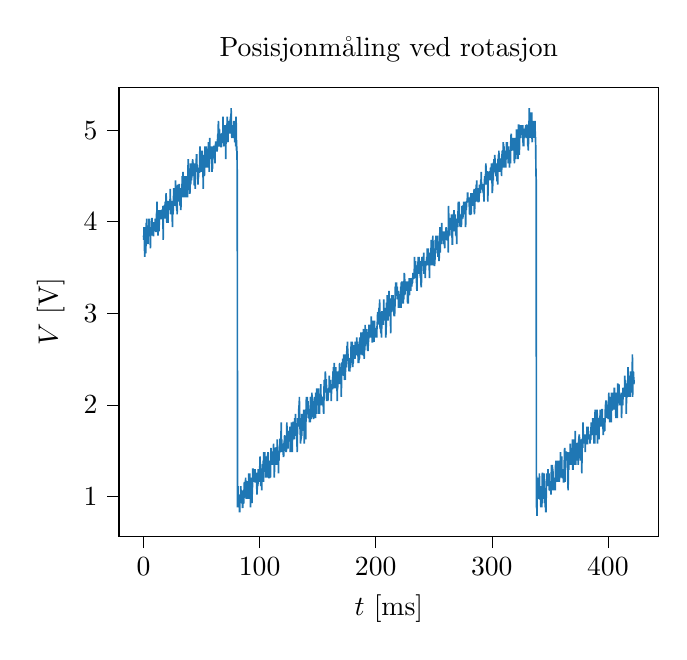
\begin{tikzpicture}

\definecolor{darkgray176}{RGB}{176,176,176}
\definecolor{steelblue31119180}{RGB}{31,119,180}

\begin{axis}[
tick align=outside,
tick pos=left,
title={Posisjonmåling ved rotasjon},
x grid style={darkgray176},
xlabel={\(\displaystyle t\) [ms]},
xmin=-21.12943, xmax=443.71803,
xtick style={color=black},
xtick={-100,0,100,200,300,400,500},
xticklabels={
  \(\displaystyle {\ensuremath{-}100}\),
  \(\displaystyle {0}\),
  \(\displaystyle {100}\),
  \(\displaystyle {200}\),
  \(\displaystyle {300}\),
  \(\displaystyle {400}\),
  \(\displaystyle {500}\)
},
y grid style={darkgray176},
ylabel={\(\displaystyle V\) [V]},
ymin=0.5644037625, ymax=5.4628464875,
ytick style={color=black},
ytick={0,1,2,3,4,5,6},
yticklabels={
  \(\displaystyle {0}\),
  \(\displaystyle {1}\),
  \(\displaystyle {2}\),
  \(\displaystyle {3}\),
  \(\displaystyle {4}\),
  \(\displaystyle {5}\),
  \(\displaystyle {6}\)
}
]
\addplot [semithick, steelblue31119180]
table {%
0 3.8485825
0.211400000000417 3.802194
0.422800000000834 3.9413595
0.634200000000362 3.8485825
0.845600000000779 3.7094265
1.05700000000031 3.6166495
1.26840000000072 3.9413595
1.47980000000025 3.802194
1.69120000000067 3.663038
1.9026000000002 3.663038
2.11400000000062 3.755815
2.32540000000014 3.987748
2.53680000000056 3.8485825
2.74820000000009 4.034127
2.95960000000051 3.894971
3.17100000000003 3.755815
3.38240000000045 3.8485825
3.59380000000087 3.802194
3.8052000000004 3.755815
4.01660000000081 3.8485825
4.22800000000034 3.8485825
4.43940000000076 3.8485825
4.65080000000029 4.034127
4.8622000000007 3.894971
5.07360000000023 3.894971
5.28500000000065 3.8485825
5.49640000000018 3.8485825
5.7078000000006 3.8485825
5.91920000000012 3.7094265
6.13060000000054 3.8485825
6.34200000000007 3.9413595
6.55340000000049 3.894971
6.76480000000002 4.034127
6.97620000000043 3.8485825
7.18760000000085 4.034127
7.39900000000038 4.034127
7.61040000000079 3.8485825
7.82180000000032 3.894971
8.03320000000074 3.894971
8.24460000000027 3.894971
8.45600000000069 3.8485825
8.66740000000021 3.8485825
8.87880000000063 3.987748
9.09020000000016 3.987748
9.30160000000058 3.894971
9.5130000000001 3.987748
9.72440000000052 3.9413595
9.93580000000005 3.9413595
10.1472000000005 4.034127
10.3586 3.987748
10.5700000000004 4.034127
10.7814000000008 3.894971
10.9928000000004 3.894971
11.2042000000008 4.0805155
11.4156000000003 4.0805155
11.6270000000007 4.219681
11.8384000000002 3.9413595
12.0498000000007 4.126904
12.2612000000002 4.034127
12.4726000000006 3.8485825
12.6840000000001 3.987748
12.8954000000006 3.987748
13.1068000000001 3.987748
13.3182000000005 3.894971
13.5296 3.987748
13.7410000000004 4.126904
13.9524000000009 4.034127
14.1638000000004 4.0805155
14.3752000000008 4.0805155
14.5866000000003 4.126904
14.7980000000008 4.0805155
15.0094000000003 4.034127
15.2208000000007 4.034127
15.4322000000002 4.034127
15.6436000000006 4.0805155
15.8550000000002 4.034127
16.0664000000006 4.126904
16.2778000000001 4.126904
16.4892000000005 4.034127
16.7006000000001 4.1732925
16.9120000000005 3.802194
17.1234 4.126904
17.3348000000004 4.034127
17.5462000000008 4.126904
17.7576000000004 4.0805155
17.9690000000008 4.1732925
18.1804000000003 4.1732925
18.3918000000007 4.034127
18.6032000000003 4.219681
18.8146000000007 4.126904
19.0260000000002 4.219681
19.2374000000006 4.1732925
19.4488000000002 4.3124485
19.6602000000006 4.1732925
19.8716000000001 4.1732925
20.0830000000005 3.987748
20.2944 4.0805155
20.5058000000005 4.126904
20.7172000000009 4.034127
20.9286000000004 4.1732925
21.1400000000008 3.987748
21.3514000000004 4.219681
21.5628000000008 4.219681
21.7742000000003 4.1732925
21.9856000000007 4.126904
22.1970000000002 4.1732925
22.4084000000007 4.219681
22.6198000000002 4.1732925
22.8312000000006 4.219681
23.0426000000001 4.358837
23.2540000000006 4.1732925
23.4654000000001 4.0805155
23.6768000000005 4.219681
23.8882 4.219681
24.0996000000004 4.219681
24.3110000000009 4.0805155
24.5224000000004 4.1732925
24.7338000000008 4.034127
24.9452000000003 3.9413595
25.1566000000008 4.126904
25.3680000000003 4.0805155
25.5794000000007 4.126904
25.7908000000002 4.219681
26.0022000000006 4.358837
26.2136000000002 4.358837
26.4250000000006 4.3124485
26.6364000000001 4.358837
26.8478000000005 4.26606
27.0592000000001 4.219681
27.2706000000005 4.1732925
27.482 4.451614
27.6934000000004 4.358837
27.9048000000008 4.26606
28.1162000000004 4.1732925
28.3276000000008 4.219681
28.5390000000003 4.126904
28.7504000000007 4.219681
28.9618000000003 4.0805155
29.1732000000007 4.358837
29.3846000000002 4.4052255
29.5960000000006 4.26606
29.8074000000002 4.219681
30.0188000000006 4.358837
30.2302000000001 4.3124485
30.4416000000005 4.219681
30.653 4.4052255
30.8644000000005 4.4052255
31.0758000000009 4.26606
31.2872000000004 4.3124485
31.4986000000008 4.1732925
31.7100000000003 4.358837
31.9214000000008 4.358837
32.1328000000003 4.126904
32.3442000000007 4.219681
32.5556000000002 4.358837
32.7670000000007 4.3124485
32.9784000000002 4.26606
33.1898000000006 4.4052255
33.4012000000001 4.4980025
33.6126000000005 4.4052255
33.8240000000001 4.26606
34.0354000000005 4.5443815
34.2468 4.358837
34.4582000000004 4.451614
34.6696000000009 4.4052255
34.8810000000004 4.358837
35.0924000000008 4.4980025
35.3038000000003 4.3124485
35.5152000000007 4.26606
35.7266000000003 4.4052255
35.9380000000007 4.4980025
36.1494000000002 4.26606
36.3608000000006 4.3124485
36.5722000000002 4.26606
36.7836000000006 4.4980025
36.9950000000001 4.358837
37.2064000000005 4.358837
37.4178000000001 4.358837
37.6292000000005 4.4052255
37.8406 4.26606
38.0520000000004 4.358837
38.2634000000008 4.5443815
38.4748000000004 4.683547
38.6862000000008 4.4980025
38.8976000000003 4.451614
39.1090000000007 4.451614
39.3204000000003 4.5443815
39.5318000000007 4.4052255
39.7432000000002 4.3124485
39.9546000000006 4.3124485
40.1660000000001 4.451614
40.3774000000006 4.6371585
40.5888000000001 4.4052255
40.8002000000005 4.5443815
41.0116 4.5443815
41.2230000000005 4.59077
41.4344000000009 4.451614
41.6458000000004 4.6371585
41.8572000000008 4.4980025
42.0686000000003 4.5443815
42.2800000000008 4.683547
42.4914000000003 4.6371585
42.7028000000007 4.6371585
42.9142000000002 4.59077
43.1256000000007 4.4980025
43.3370000000002 4.59077
43.5484000000006 4.59077
43.7598000000001 4.4052255
43.9712000000005 4.4052255
44.1826000000001 4.6371585
44.3940000000005 4.59077
44.6054 4.358837
44.8168000000004 4.59077
45.0282000000009 4.5443815
45.2396000000004 4.59077
45.4510000000008 4.683547
45.6624000000003 4.7299355
45.8738000000007 4.7299355
46.0852000000003 4.5443815
46.2966000000007 4.59077
46.5080000000002 4.5443815
46.7194000000006 4.59077
46.9308000000002 4.4052255
47.1422000000006 4.4980025
47.3536000000001 4.4980025
47.5650000000005 4.59077
47.7764000000001 4.5443815
47.9878000000005 4.5443815
48.1992 4.5443815
48.4106000000004 4.7299355
48.6220000000008 4.822703
48.8334000000004 4.59077
49.0448000000008 4.7299355
49.2562000000003 4.7299355
49.4676000000007 4.683547
49.6790000000003 4.59077
49.8904000000007 4.5443815
50.1018000000002 4.59077
50.3132000000006 4.7763145
50.5246000000001 4.5443815
50.7360000000006 4.59077
50.9474000000001 4.5443815
51.1588000000005 4.7299355
51.3702 4.358837
51.5816000000004 4.5443815
51.7930000000009 4.683547
52.0044000000004 4.7299355
52.2158000000008 4.6371585
52.4272000000003 4.4980025
52.6386000000008 4.59077
52.8500000000003 4.822703
53.0614000000007 4.59077
53.2728000000002 4.683547
53.4842000000006 4.683547
53.6956000000002 4.7299355
53.9070000000006 4.683547
54.1184000000001 4.822703
54.3298000000005 4.7299355
54.5412000000001 4.6371585
54.7526000000005 4.59077
54.964 4.6371585
55.1754000000004 4.59077
55.3868000000008 4.6371585
55.5982000000004 4.59077
55.8096000000008 4.683547
56.0210000000003 4.8690915
56.2324000000007 4.7299355
56.4438000000003 4.822703
56.6552000000007 4.5443815
56.8666000000002 4.7299355
57.0780000000006 4.91548
57.2894000000002 4.7299355
57.5008000000006 4.683547
57.7122000000001 4.7763145
57.9236000000005 4.822703
58.135 4.683547
58.3464000000005 4.822703
58.5578 4.7763145
58.7692000000004 4.822703
58.9806000000008 4.5443815
59.1920000000004 4.59077
59.4034000000008 4.59077
59.6148000000003 4.7299355
59.8262000000007 4.822703
60.0376000000002 4.7299355
60.2490000000007 4.7299355
60.4604000000002 4.7763145
60.6718000000006 4.822703
60.8832000000001 4.822703
61.0946000000006 4.7763145
61.3060000000001 4.7299355
61.5174000000005 4.6371585
61.7288 4.7763145
61.9402000000004 4.822703
62.1516000000009 4.8690915
62.3630000000004 4.8690915
62.5744000000008 4.8690915
62.7858000000003 4.7763145
62.9972000000008 4.7763145
63.2086000000003 4.7763145
63.4200000000007 4.7763145
63.6314000000002 4.8690915
63.8428000000006 4.91548
64.0542000000002 4.9618685
64.2656000000006 4.91548
64.4770000000001 5.1010245
64.6884000000005 5.054636
64.8998000000001 4.8690915
65.1112000000005 4.822703
65.3226 4.8690915
65.5340000000004 5.0082475
65.7454000000008 4.822703
65.9568000000004 4.91548
66.1682000000008 4.8690915
66.3796000000003 4.9618685
66.5910000000007 4.822703
66.8024000000003 4.822703
67.0138000000007 4.822703
67.2252000000002 4.91548
67.4366000000006 4.91548
67.6480000000002 4.9618685
67.8594000000006 4.9618685
68.0708000000001 4.91548
68.2822000000005 4.8690915
68.4936 5.147413
68.7050000000005 4.91548
68.9164000000009 4.8690915
69.1278000000004 4.822703
69.3392000000008 4.9618685
69.5506000000003 4.8690915
69.7620000000008 4.91548
69.9734000000003 5.054636
70.1848000000007 4.8690915
70.3962000000002 4.9618685
70.6076000000007 4.9618685
70.8190000000002 4.683547
71.0304000000006 4.91548
71.2418000000001 5.0082475
71.4532000000005 4.9618685
71.6646000000001 5.054636
71.8760000000005 5.0082475
72.0874 5.147413
72.2988000000004 4.9618685
72.5102000000009 4.91548
72.7216000000004 4.8690915
72.9330000000008 5.1010245
73.1444000000003 5.054636
73.3558000000008 4.9618685
73.5672000000003 5.054636
73.7786000000007 5.054636
73.9900000000002 4.9618685
74.2014000000006 5.054636
74.4128000000002 4.9618685
74.6242000000006 5.054636
74.8356000000001 5.147413
75.0470000000005 5.0082475
75.2584000000001 5.0082475
75.4698000000005 5.24019
75.6812 5.0082475
75.8926000000004 4.9618685
76.1040000000008 4.91548
76.3154000000004 5.054636
76.5268000000008 4.9618685
76.7382000000003 5.054636
76.9496000000007 4.91548
77.1610000000003 4.9618685
77.3724000000007 5.0082475
77.5838000000002 5.0082475
77.7952000000006 5.1010245
78.0066000000001 5.054636
78.2180000000006 4.9618685
78.4294000000001 4.91548
78.6408000000005 4.8690915
78.8522 5.054636
79.0636000000005 4.8690915
79.2750000000009 5.1010245
79.4864000000004 4.822703
79.6978000000008 5.147413
79.9092000000003 5.0082475
80.1206000000008 4.7763145
80.3320000000003 4.822703
80.5434000000007 4.7299355
80.7548000000002 4.451614
80.9662000000007 0.8798344
81.1776000000002 1.0653808
81.3890000000006 1.1117674
81.6004000000001 0.9726076
81.8118000000005 0.9726076
82.0232000000001 0.926221
82.2346000000005 0.9726076
82.446 0.9726076
82.6574000000004 0.83344685
82.8688000000008 0.83344685
83.0802000000004 1.0189942
83.2916000000008 0.9726076
83.5030000000003 0.926221
83.7144000000008 1.1117674
83.9258000000003 1.0653808
84.1372000000007 1.0189942
84.3486000000002 0.926221
84.5600000000006 0.9726076
84.7714000000002 0.9726076
84.9828000000006 0.9726076
85.1942000000001 0.8798344
85.4056000000005 0.8798344
85.617 1.0653808
85.8284000000005 0.926221
86.0398 0.926221
86.2512000000004 0.926221
86.4626000000008 0.9726076
86.6740000000004 1.1117674
86.8854000000008 1.158154
87.0968000000003 1.1117674
87.3082000000007 1.158154
87.5196000000003 1.1117674
87.7310000000007 1.0653808
87.9424000000002 1.2045406
88.1538000000006 1.0653808
88.3652000000001 0.9726076
88.5766000000006 1.1117674
88.7880000000001 1.1117674
88.9994000000005 1.158154
89.2108 1.158154
89.4222000000005 1.0653808
89.6336000000009 1.1117674
89.8450000000004 1.0653808
90.0564000000008 0.9726076
90.2678000000003 1.1117674
90.4792000000008 1.0189942
90.6906000000003 1.250931
90.9020000000007 1.1117674
91.1134000000002 1.0189942
91.3248000000006 0.9726076
91.5362000000002 1.250931
91.7476000000006 1.0189942
91.9590000000001 1.1117674
92.1704000000005 0.8798344
92.3818000000001 1.2045406
92.5932000000005 1.158154
92.8046 1.0653808
93.0160000000004 1.1117674
93.2274000000008 1.0189942
93.4388000000004 0.926221
93.6502000000008 1.0653808
93.8616000000003 1.1117674
94.0730000000007 1.29731
94.2844000000003 1.29731
94.4958000000007 1.2045406
94.7072000000002 1.250931
94.9186000000006 1.2045406
95.1300000000002 1.29731
95.3414000000006 1.158154
95.5528000000001 1.2045406
95.7642000000005 1.2045406
95.9756 1.29731
96.1870000000005 1.158154
96.3984 1.158154
96.6098000000004 1.2045406
96.8212000000008 1.2045406
97.0326000000004 1.250931
97.2440000000008 1.250931
97.4554000000003 1.2045406
97.6668000000007 1.0189942
97.8782000000002 1.0653808
98.0896000000007 1.2045406
98.3010000000002 1.250931
98.5124000000006 1.1117674
98.7238000000001 1.29731
98.9352000000005 1.158154
99.1466000000001 1.2045406
99.3580000000005 1.158154
99.5694 1.250931
99.7808000000005 1.2045406
99.9922000000009 1.2045406
100.2036 1.3436985
100.415000000001 1.4364755
100.6264 1.2045406
100.837800000001 1.250931
101.0492 1.1117674
101.260600000001 1.158154
101.472 1.158154
101.683400000001 1.158154
101.8948 1.0653808
102.106200000001 1.29731
102.3176 1.29731
102.529000000001 1.3436985
102.7404 1.3436985
102.9518 1.29731
103.1632 1.390087
103.3746 1.158154
103.586000000001 1.482864
103.7974 1.3436985
104.008800000001 1.29731
104.2202 1.3436985
104.431600000001 1.482864
104.643 1.3436985
104.854400000001 1.29731
105.0658 1.29731
105.277200000001 1.2045406
105.4886 1.4364755
105.700000000001 1.2045406
105.9114 1.29731
106.122800000001 1.3436985
106.3342 1.3436985
106.5456 1.2045406
106.757000000001 1.4364755
106.9684 1.4364755
107.179800000001 1.482864
107.3912 1.29731
107.602600000001 1.29731
107.814 1.3436985
108.025400000001 1.2045406
108.2368 1.2045406
108.448200000001 1.2045406
108.6596 1.390087
108.871000000001 1.2045406
109.0824 1.3436985
109.293800000001 1.2045406
109.5052 1.3436985
109.7166 1.5292525
109.928 1.482864
110.1394 1.482864
110.350800000001 1.3436985
110.5622 1.482864
110.773600000001 1.482864
110.985 1.4364755
111.196400000001 1.4364755
111.4078 1.3436985
111.619200000001 1.482864
111.8306 1.4364755
112.042000000001 1.5756315
112.2534 1.4364755
112.464800000001 1.3436985
112.6762 1.2045406
112.887600000001 1.390087
113.099 1.482864
113.3104 1.3436985
113.5218 1.390087
113.7332 1.482864
113.944600000001 1.5292525
114.156 1.4364755
114.367400000001 1.5292525
114.5788 1.5292525
114.790200000001 1.3436985
115.0016 1.390087
115.213000000001 1.62202
115.4244 1.482864
115.635800000001 1.482864
115.8472 1.4364755
116.058600000001 1.4364755
116.27 1.250931
116.481400000001 1.482864
116.6928 1.390087
116.9042 1.482864
117.115600000001 1.482864
117.327 1.5292525
117.538400000001 1.62202
117.7498 1.62202
117.961200000001 1.5292525
118.1726 1.62202
118.384000000001 1.62202
118.5954 1.8075645
118.806800000001 1.482864
119.0182 1.62202
119.229600000001 1.5292525
119.441 1.5292525
119.652400000001 1.5292525
119.8638 1.5756315
120.0752 1.5292525
120.2866 1.482864
120.498 1.4364755
120.709400000001 1.4364755
120.9208 1.5756315
121.132200000001 1.5756315
121.3436 1.62202
121.555000000001 1.6684085
121.7664 1.5756315
121.977800000001 1.5756315
122.1892 1.62202
122.400600000001 1.5756315
122.612 1.482864
122.823400000001 1.62202
123.0348 1.482864
123.246200000001 1.5756315
123.4576 1.8075645
123.669 1.6684085
123.8804 1.5292525
124.0918 1.5292525
124.303200000001 1.5292525
124.5146 1.5292525
124.726000000001 1.714797
124.9374 1.62202
125.148800000001 1.714797
125.3602 1.62202
125.571600000001 1.714797
125.783 1.6684085
125.994400000001 1.714797
126.2058 1.7611855
126.417200000001 1.482864
126.6286 1.714797
126.840000000001 1.62202
127.0514 1.6684085
127.2628 1.6684085
127.474200000001 1.8075645
127.6856 1.6684085
127.897000000001 1.6684085
128.1084 1.482864
128.319800000001 1.6684085
128.5312 1.6684085
128.742600000001 1.714797
128.954 1.8075645
129.165400000001 1.8075645
129.3768 1.8075645
129.588200000001 1.8075645
129.7996 1.62202
130.011000000001 1.7611855
130.2224 1.853953
130.4338 1.6684085
130.6452 1.6684085
130.8566 1.9003415
131.068000000001 1.6684085
131.2794 1.6684085
131.490800000001 1.6684085
131.7022 1.7611855
131.913600000001 1.62202
132.125 1.6684085
132.336400000001 1.482864
132.5478 1.6684085
132.759200000001 1.853953
132.9706 1.8075645
133.182000000001 1.7611855
133.3934 1.8075645
133.604800000001 1.8075645
133.8162 1.9931185
134.0276 1.8075645
134.239 2.085886
134.4504 1.853953
134.661800000001 1.9003415
134.8732 1.714797
135.084600000001 1.6684085
135.296 1.5756315
135.507400000001 1.6684085
135.7188 1.62202
135.930200000001 1.6684085
136.1416 1.6684085
136.353000000001 1.6684085
136.5644 1.9003415
136.775800000001 1.853953
136.9872 1.853953
137.198600000001 1.853953
137.41 1.853953
137.6214 1.8075645
137.832800000001 1.714797
138.0442 1.94673
138.255600000001 1.853953
138.467 1.5756315
138.678400000001 1.8075645
138.8898 1.94673
139.101200000001 1.7611855
139.3126 1.7611855
139.524000000001 1.7611855
139.7354 1.62202
139.946800000001 1.9003415
140.1582 2.0394975
140.369600000001 2.085886
140.581 1.853953
140.7924 1.9931185
141.0038 2.085886
141.2152 1.94673
141.426600000001 1.9931185
141.638 2.0394975
141.849400000001 1.9003415
142.0608 1.94673
142.272200000001 1.94673
142.4836 1.853953
142.695000000001 1.9003415
142.9064 1.8075645
143.117800000001 1.9003415
143.3292 1.94673
143.540600000001 1.8075645
143.752 2.085886
143.963400000001 1.9003415
144.1748 1.853953
144.3862 1.853953
144.597600000001 1.94673
144.809 1.9931185
145.020400000001 2.1322745
145.2318 1.9931185
145.443200000001 1.9931185
145.6546 2.085886
145.866000000001 1.9931185
146.0774 1.94673
146.288800000001 1.853953
146.5002 1.853953
146.711600000001 2.0394975
146.923 1.9003415
147.134400000001 1.853953
147.3458 1.9003415
147.557200000001 1.853953
147.7686 2.085886
147.98 2.0394975
148.191400000001 1.853953
148.4028 2.1322745
148.614200000001 1.94673
148.8256 1.9931185
149.037000000001 1.9003415
149.2484 2.178663
149.459800000001 2.085886
149.6712 1.9931185
149.882600000001 2.1322745
150.094 1.9931185
150.305400000001 2.178663
150.5168 1.9931185
150.728200000001 2.085886
150.9396 1.9003415
151.151 1.94673
151.3624 1.94673
151.5738 1.9003415
151.785200000001 2.0394975
151.9966 2.085886
152.208000000001 2.178663
152.4194 1.9931185
152.630800000001 2.2250515
152.8422 2.085886
153.053600000001 2.085886
153.265 2.085886
153.476400000001 2.0394975
153.6878 2.0394975
153.899200000001 1.9931185
154.1106 2.0394975
154.322000000001 2.085886
154.5334 2.0394975
154.7448 2.0394975
154.956200000001 1.94673
155.1676 1.9003415
155.379000000001 2.0394975
155.5904 2.27144
155.801800000001 2.1322745
156.0132 2.178663
156.224600000001 2.1322745
156.436 2.317819
156.647400000001 2.3642075
156.8588 2.2250515
157.070200000001 2.178663
157.2816 2.27144
157.493000000001 2.27144
157.7044 2.0394975
157.915800000001 2.178663
158.1272 2.0394975
158.3386 2.178663
158.550000000001 2.085886
158.7614 2.0394975
158.972800000001 2.085886
159.1842 2.1322745
159.395600000001 2.178663
159.607 2.1322745
159.818400000001 2.178663
160.0298 2.317819
160.241200000001 2.178663
160.4526 2.1322745
160.664000000001 2.27144
160.8754 2.178663
161.086800000001 2.27144
161.2982 2.178663
161.5096 2.2250515
161.721 2.0394975
161.9324 2.178663
162.143800000001 2.178663
162.3552 2.178663
162.566600000001 2.178663
162.778 2.178663
162.989400000001 2.27144
163.2008 2.3642075
163.412200000001 2.178663
163.6236 2.410596
163.835000000001 2.317819
164.0464 2.27144
164.257800000001 2.4569845
164.4692 2.3642075
164.680600000001 2.178663
164.892 2.410596
165.1034 2.2250515
165.314800000001 2.317819
165.5262 2.410596
165.737600000001 2.27144
165.949 2.317819
166.160400000001 2.178663
166.3718 2.27144
166.583200000001 2.3642075
166.7946 2.0394975
167.006000000001 2.178663
167.2174 2.178663
167.428800000001 2.3642075
167.6402 2.317819
167.851600000001 2.2250515
168.063 2.317819
168.2744 2.317819
168.4858 2.3642075
168.6972 2.3642075
168.908600000001 2.4569845
169.12 2.410596
169.331400000001 2.2250515
169.5428 2.317819
169.754200000001 2.3642075
169.9656 2.2250515
170.177000000001 2.27144
170.3884 2.085886
170.599800000001 2.3642075
170.8112 2.410596
171.022600000001 2.4569845
171.234 2.4569845
171.445400000001 2.317819
171.6568 2.503373
171.8682 2.4569845
172.0796 2.317819
172.291 2.3642075
172.502400000001 2.549752
172.7138 2.4569845
172.925200000001 2.4569845
173.1366 2.27144
173.348000000001 2.549752
173.5594 2.317819
173.770800000001 2.27144
173.9822 2.410596
174.193600000001 2.549752
174.405 2.4569845
174.616400000001 2.410596
174.8278 2.4569845
175.039200000001 2.549752
175.2506 2.642529
175.462 2.503373
175.673400000001 2.6889175
175.8848 2.5961405
176.096200000001 2.549752
176.3076 2.503373
176.519000000001 2.503373
176.7304 2.4569845
176.941800000001 2.3642075
177.1532 2.503373
177.364600000001 2.503373
177.576 2.3642075
177.787400000001 2.410596
177.9988 2.410596
178.210200000001 2.410596
178.4216 2.503373
178.633 2.503373
178.8444 2.6889175
179.0558 2.4569845
179.267200000001 2.642529
179.4786 2.549752
179.690000000001 2.6889175
179.9014 2.642529
180.112800000001 2.549752
180.3242 2.410596
180.535600000001 2.5961405
180.747 2.4569845
180.958400000001 2.642529
181.1698 2.642529
181.381200000001 2.549752
181.5926 2.5961405
181.804000000001 2.503373
182.0154 2.642529
182.2268 2.503373
182.4382 2.6889175
182.6496 2.5961405
182.861000000001 2.549752
183.0724 2.549752
183.283800000001 2.549752
183.4952 2.549752
183.706600000001 2.735306
183.918 2.549752
184.129400000001 2.5961405
184.3408 2.6889175
184.552200000001 2.642529
184.7636 2.549752
184.975000000001 2.4569845
185.1864 2.549752
185.397800000001 2.4569845
185.6092 2.503373
185.8206 2.5961405
186.032000000001 2.503373
186.2434 2.735306
186.454800000001 2.549752
186.6662 2.642529
186.877600000001 2.642529
187.089 2.549752
187.300400000001 2.781685
187.5118 2.781685
187.723200000001 2.642529
187.9346 2.5961405
188.146000000001 2.6889175
188.3574 2.781685
188.568800000001 2.549752
188.7802 2.549752
188.9916 2.6889175
189.203 2.735306
189.4144 2.8280735
189.625800000001 2.6889175
189.8372 2.5961405
190.048600000001 2.503373
190.26 2.5961405
190.471400000001 2.5961405
190.6828 2.642529
190.894200000001 2.874462
191.1056 2.642529
191.317000000001 2.781685
191.5284 2.6889175
191.739800000001 2.781685
191.9512 2.735306
192.162600000001 2.6889175
192.374 2.8280735
192.5854 2.6889175
192.796800000001 2.6889175
193.0082 2.5961405
193.219600000001 2.5961405
193.431 2.5961405
193.642400000001 2.735306
193.8538 2.6889175
194.065200000001 2.781685
194.2766 2.874462
194.488000000001 2.781685
194.6994 2.8280735
194.910800000001 2.874462
195.1222 2.8280735
195.333600000001 2.874462
195.545 2.735306
195.7564 2.8280735
195.9678 2.735306
196.1792 2.967239
196.390600000001 2.8280735
196.602 2.874462
196.813400000001 2.781685
197.0248 2.6889175
197.236200000001 2.6889175
197.4476 2.781685
197.659000000001 2.8280735
197.8704 2.9208505
198.081800000001 2.8280735
198.2932 2.874462
198.504600000001 2.6889175
198.716 2.781685
198.927400000001 2.9208505
199.1388 2.8280735
199.3502 2.8280735
199.5616 2.8280735
199.773 2.735306
199.984400000001 2.781685
200.1958 2.8280735
200.407200000001 2.8280735
200.6186 2.781685
200.830000000001 2.735306
201.0414 2.8280735
201.252800000001 2.874462
201.4642 2.9208505
201.675600000001 3.0136275
201.887 2.9208505
202.098400000001 2.967239
202.3098 2.967239
202.521200000001 2.9208505
202.7326 3.0600065
202.944 2.9208505
203.155400000001 2.874462
203.3668 3.1527835
203.578200000001 2.967239
203.7896 2.8280735
204.001000000001 2.874462
204.2124 2.9208505
204.423800000001 2.781685
204.6352 2.9208505
204.846600000001 2.9208505
205.058 2.735306
205.269400000001 3.0136275
205.4808 3.0136275
205.692200000001 2.967239
205.9036 2.9208505
206.115 3.0136275
206.3264 2.9208505
206.5378 2.874462
206.749200000001 2.967239
206.9606 3.1527835
207.172000000001 2.967239
207.3834 2.9208505
207.594800000001 2.967239
207.8062 2.9208505
208.017600000001 2.967239
208.229 3.0600065
208.440400000001 3.0136275
208.6518 2.735306
208.863200000001 2.781685
209.0746 2.874462
209.286000000001 3.106395
209.4974 3.106395
209.7088 3.0600065
209.9202 3.199172
210.1316 3.0136275
210.343000000001 3.1527835
210.5544 2.9208505
210.765800000001 3.0600065
210.9772 3.106395
211.188600000001 3.0136275
211.4 3.2455605
211.611400000001 3.0136275
211.8228 3.0600065
212.034200000001 2.967239
212.2456 3.106395
212.457000000001 2.967239
212.6684 3.0136275
212.879800000001 2.781685
213.0912 3.1527835
213.3026 3.1527835
213.514000000001 3.0136275
213.7254 3.199172
213.936800000001 3.106395
214.1482 3.0600065
214.359600000001 3.199172
214.571 3.0600065
214.782400000001 3.0600065
214.9938 3.199172
215.205200000001 3.0136275
215.4166 3.0600065
215.628000000001 3.106395
215.8394 2.967239
216.050800000001 3.0600065
216.2622 2.967239
216.4736 3.0600065
216.685 3.106395
216.8964 3.2919395
217.107800000001 3.1527835
217.3192 3.338328
217.530600000001 3.199172
217.742 3.199172
217.953400000001 3.338328
218.1648 3.199172
218.376200000001 3.199172
218.5876 3.2919395
218.799000000001 3.199172
219.0104 3.1527835
219.221800000001 3.199172
219.4332 3.2455605
219.644600000001 3.0600065
219.856 3.199172
220.0674 3.0600065
220.2788 3.1527835
220.4902 3.106395
220.701600000001 3.1527835
220.913 3.199172
221.124400000001 3.199172
221.3358 3.199172
221.547200000001 3.2919395
221.7586 3.0600065
221.970000000001 3.338328
222.1814 3.2919395
222.392800000001 3.106395
222.6042 3.338328
222.815600000001 3.338328
223.027 3.199172
223.2384 3.199172
223.4498 3.2919395
223.6612 3.106395
223.872600000001 3.199172
224.084 3.1527835
224.295400000001 3.199172
224.5068 3.431105
224.718200000001 3.431105
224.9296 3.3847165
225.141000000001 3.199172
225.3524 3.338328
225.563800000001 3.338328
225.7752 3.338328
225.986600000001 3.338328
226.198 3.338328
226.409400000001 3.338328
226.6208 3.2455605
226.8322 3.338328
227.0436 3.338328
227.255 3.338328
227.466400000001 3.106395
227.6778 3.2455605
227.889200000001 3.338328
228.1006 3.106395
228.312000000001 3.338328
228.5234 3.338328
228.734800000001 3.2919395
228.9462 3.3847165
229.157600000001 3.199172
229.369 3.338328
229.580400000001 3.338328
229.7918 3.3847165
230.003200000001 3.338328
230.2146 3.2455605
230.426 3.338328
230.637400000001 3.338328
230.8488 3.3847165
231.060200000001 3.2919395
231.2716 3.338328
231.483000000001 3.338328
231.6944 3.338328
231.905800000001 3.3847165
232.1172 3.431105
232.328600000001 3.431105
232.54 3.3847165
232.751400000001 3.3847165
232.9628 3.431105
233.174200000001 3.3847165
233.3856 3.6166495
233.597 3.3847165
233.8084 3.5238725
234.0198 3.431105
234.231200000001 3.570261
234.4426 3.5238725
234.654000000001 3.4774935
234.8654 3.4774935
235.076800000001 3.3847165
235.2882 3.2919395
235.499600000001 3.2455605
235.711 3.3847165
235.922400000001 3.431105
236.1338 3.5238725
236.345200000001 3.431105
236.5566 3.6166495
236.768000000001 3.431105
236.9794 3.570261
237.1908 3.4774935
237.4022 3.6166495
237.6136 3.431105
237.825000000001 3.4774935
238.0364 3.431105
238.247800000001 3.570261
238.4592 3.3847165
238.670600000001 3.5238725
238.882 3.4774935
239.093400000001 3.2919395
239.3048 3.2919395
239.516200000001 3.431105
239.7276 3.5238725
239.939000000001 3.6166495
240.1504 3.5238725
240.361800000001 3.5238725
240.5732 3.570261
240.7846 3.6166495
240.996000000001 3.570261
241.2074 3.6166495
241.418800000001 3.663038
241.6302 3.431105
241.841600000001 3.570261
242.053 3.5238725
242.264400000001 3.5238725
242.4758 3.570261
242.687200000001 3.3847165
242.8986 3.5238725
243.110000000001 3.5238725
243.3214 3.570261
243.532800000001 3.5238725
243.7442 3.570261
243.9556 3.6166495
244.167 3.5238725
244.3784 3.7094265
244.589800000001 3.570261
244.8012 3.6166495
245.012600000001 3.570261
245.224 3.7094265
245.435400000001 3.570261
245.6468 3.5238725
245.858200000001 3.570261
246.0696 3.570261
246.281000000001 3.3847165
246.4924 3.663038
246.703800000001 3.5238725
246.9152 3.570261
247.126600000001 3.5238725
247.338 3.570261
247.5494 3.5238725
247.7608 3.802194
247.9722 3.6166495
248.183600000001 3.7094265
248.395 3.5238725
248.606400000001 3.755815
248.8178 3.755815
249.029200000001 3.755815
249.2406 3.8485825
249.452000000001 3.5238725
249.6634 3.663038
249.874800000001 3.663038
250.0862 3.7094265
250.297600000001 3.663038
250.509 3.5238725
250.7204 3.5238725
250.9318 3.570261
251.1432 3.6166495
251.354600000001 3.802194
251.566 3.663038
251.777400000001 3.663038
251.9888 3.8485825
252.200200000001 3.7094265
252.4116 3.755815
252.623000000001 3.7094265
252.8344 3.7094265
253.045800000001 3.802194
253.2572 3.8485825
253.468600000001 3.7094265
253.68 3.6166495
253.891400000001 3.755815
254.1028 3.663038
254.3142 3.663038
254.5256 3.570261
254.737 3.6166495
254.948400000001 3.755815
255.1598 3.8485825
255.371200000001 3.9413595
255.5826 3.663038
255.794000000001 3.8485825
256.0054 3.8485825
256.216800000001 3.755815
256.4282 3.8485825
256.639600000001 3.8485825
256.851 3.987748
257.062400000001 3.802194
257.2738 3.8485825
257.485200000001 3.802194
257.6966 3.894971
257.908 3.8485825
258.1194 3.755815
258.3308 3.802194
258.542200000001 3.894971
258.7536 3.755815
258.965000000001 3.802194
259.1764 3.802194
259.387800000001 3.7094265
259.5992 3.802194
259.810600000001 3.8485825
260.022 3.894971
260.233400000001 3.802194
260.4448 3.894971
260.656200000001 3.9413595
260.8676 3.894971
261.079000000001 3.894971
261.2904 3.8485825
261.5018 3.802194
261.713200000001 3.802194
261.9246 3.894971
262.136000000001 3.802194
262.3474 3.8485825
262.558800000001 3.663038
262.7702 4.1732925
262.981600000001 3.9413595
263.193 4.034127
263.404400000001 3.987748
263.6158 3.894971
263.827200000001 3.8485825
264.0386 3.987748
264.250000000001 4.034127
264.4614 4.034127
264.672800000001 3.9413595
264.8842 3.9413595
265.0956 3.987748
265.307000000001 4.0805155
265.5184 3.9413595
265.729800000001 3.8485825
265.9412 3.755815
266.152600000001 3.755815
266.364 4.0805155
266.575400000001 3.987748
266.7868 4.034127
266.998200000001 3.894971
267.2096 4.0805155
267.421000000001 4.126904
267.6324 4.034127
267.8438 4.034127
268.0552 4.034127
268.2666 3.987748
268.478 4.0805155
268.6894 3.9413595
268.900800000001 3.8485825
269.1122 3.9413595
269.323600000001 4.034127
269.535 3.9413595
269.746400000001 3.755815
269.9578 3.987748
270.169200000001 3.987748
270.3806 3.987748
270.592000000001 3.9413595
270.8034 3.987748
271.014800000001 4.1732925
271.2262 4.219681
271.4376 4.034127
271.649 3.987748
271.8604 4.219681
272.071800000001 4.0805155
272.2832 4.0805155
272.494600000001 4.034127
272.706 3.9413595
272.917400000001 3.987748
273.1288 4.034127
273.340200000001 4.034127
273.5516 4.0805155
273.763000000001 3.9413595
273.9744 4.034127
274.185800000001 4.034127
274.3972 4.1732925
274.608600000001 4.0805155
274.82 4.126904
275.0314 4.034127
275.2428 4.0805155
275.4542 4.1732925
275.665600000001 4.1732925
275.877 4.219681
276.088400000001 4.126904
276.2998 4.1732925
276.511200000001 4.0805155
276.7226 4.219681
276.934000000001 4.126904
277.1454 4.219681
277.356800000001 3.9413595
277.5682 3.987748
277.779600000001 4.219681
277.991 4.126904
278.202400000001 4.1732925
278.4138 4.219681
278.6252 4.219681
278.836600000001 4.219681
279.048 4.3124485
279.259400000001 4.3124485
279.4708 4.219681
279.682200000001 4.219681
279.8936 4.26606
280.105000000001 4.219681
280.3164 4.219681
280.527800000001 4.26606
280.7392 4.0805155
280.950600000001 4.219681
281.162 4.219681
281.373400000001 4.0805155
281.5848 4.0805155
281.796200000001 4.219681
282.0076 4.3124485
282.219 4.0805155
282.430400000001 4.219681
282.6418 4.219681
282.853200000001 4.3124485
283.0646 4.219681
283.276000000001 4.219681
283.4874 4.219681
283.698800000001 4.1732925
283.9102 4.26606
284.121600000001 4.3124485
284.333 4.26606
284.544400000001 4.219681
284.7558 4.358837
284.967200000001 4.0805155
285.1786 4.126904
285.39 4.1732925
285.6014 4.3124485
285.8128 4.26606
286.024200000001 4.3124485
286.2356 4.358837
286.447000000001 4.358837
286.6584 4.4052255
286.869800000001 4.26606
287.0812 4.451614
287.292600000001 4.219681
287.504 4.26606
287.715400000001 4.26606
287.9268 4.358837
288.138200000001 4.358837
288.3496 4.219681
288.561 4.219681
288.7724 4.358837
288.9838 4.219681
289.195200000001 4.3124485
289.4066 4.4052255
289.618000000001 4.358837
289.8294 4.4052255
290.040800000001 4.358837
290.2522 4.3124485
290.463600000001 4.451614
290.675 4.4052255
290.886400000001 4.5443815
291.0978 4.4052255
291.309200000001 4.358837
291.5206 4.358837
291.732000000001 4.4052255
291.9434 4.4052255
292.1548 4.358837
292.3662 4.358837
292.5776 4.3124485
292.789000000001 4.358837
293.0004 4.358837
293.211800000001 4.219681
293.4232 4.4052255
293.634600000001 4.4052255
293.846 4.4980025
294.057400000001 4.4052255
294.2688 4.4980025
294.480200000001 4.451614
294.6916 4.5443815
294.903000000001 4.6371585
295.1144 4.451614
295.325800000001 4.4052255
295.5372 4.5443815
295.7486 4.4980025
295.96 4.5443815
296.1714 4.5443815
296.382800000001 4.451614
296.5942 4.219681
296.805600000001 4.451614
297.017 4.5443815
297.228400000001 4.451614
297.4398 4.4980025
297.651200000001 4.451614
297.8626 4.4980025
298.074000000001 4.5443815
298.2854 4.5443815
298.496800000001 4.5443815
298.7082 4.4980025
298.919600000001 4.59077
299.131 4.4980025
299.3424 4.451614
299.553800000001 4.59077
299.7652 4.6371585
299.976600000001 4.4980025
300.188 4.451614
300.399400000001 4.3124485
300.6108 4.358837
300.822200000001 4.4052255
301.0336 4.5443815
301.245000000001 4.451614
301.4564 4.6371585
301.667800000001 4.6371585
301.8792 4.683547
302.090600000001 4.5443815
302.302 4.6371585
302.513400000001 4.7299355
302.7248 4.683547
302.9362 4.6371585
303.147600000001 4.5443815
303.359 4.5443815
303.570400000001 4.4980025
303.7818 4.5443815
303.993200000001 4.6371585
304.2046 4.5443815
304.416000000001 4.451614
304.6274 4.451614
304.838800000001 4.59077
305.0502 4.4052255
305.261600000001 4.683547
305.473 4.59077
305.684400000001 4.7299355
305.8958 4.6371585
306.1072 4.7763145
306.3186 4.5443815
306.53 4.59077
306.741400000001 4.59077
306.9528 4.5443815
307.164200000001 4.59077
307.3756 4.683547
307.587000000001 4.683547
307.7984 4.59077
308.009800000001 4.6371585
308.2212 4.683547
308.432600000001 4.4980025
308.644 4.7299355
308.855400000001 4.7299355
309.0668 4.7763145
309.2782 4.7299355
309.4896 4.683547
309.701 4.7763145
309.912400000001 4.8690915
310.1238 4.822703
310.335200000001 4.59077
310.5466 4.822703
310.758000000001 4.7299355
310.9694 4.7299355
311.180800000001 4.7299355
311.3922 4.7299355
311.603600000001 4.683547
311.815 4.7763145
312.026400000001 4.59077
312.2378 4.7299355
312.449200000001 4.683547
312.6606 4.8690915
312.872 4.7299355
313.0834 4.822703
313.2948 4.8690915
313.506200000001 4.7299355
313.7176 4.7763145
313.929000000001 4.822703
314.1404 4.6371585
314.351800000001 4.7299355
314.5632 4.7763145
314.774600000001 4.7763145
314.986 4.7299355
315.197400000001 4.59077
315.4088 4.7299355
315.620200000001 4.7299355
315.8316 4.822703
316.043000000001 4.6371585
316.2544 4.822703
316.4658 4.91548
316.677200000001 4.9618685
316.8886 4.8690915
317.100000000001 4.8690915
317.3114 4.91548
317.522800000001 4.822703
317.7342 4.7763145
317.945600000001 4.8690915
318.157 4.822703
318.368400000001 4.8690915
318.5798 4.91548
318.791200000001 4.822703
319.0026 4.8690915
319.214000000001 4.91548
319.4254 4.6371585
319.636800000001 4.683547
319.8482 4.8690915
320.0596 4.7763145
320.271000000001 4.7299355
320.4824 4.7763145
320.693800000001 4.683547
320.9052 4.91548
321.116600000001 4.7299355
321.328 5.0082475
321.539400000001 4.9618685
321.7508 4.91548
321.962200000001 4.7763145
322.1736 4.91548
322.385000000001 4.9618685
322.5964 4.683547
322.807800000001 4.7763145
323.0192 5.054636
323.2306 5.054636
323.442 4.7763145
323.6534 4.7299355
323.864800000001 4.822703
324.0762 5.054636
324.287600000001 4.9618685
324.499 4.9618685
324.710400000001 5.0082475
324.9218 4.91548
325.133200000001 4.9618685
325.3446 5.054636
325.556000000001 5.0082475
325.7674 5.0082475
325.978800000001 4.9618685
326.1902 4.9618685
326.4016 5.0082475
326.613 5.054636
326.8244 4.91548
327.035800000001 4.822703
327.2472 4.91548
327.458600000001 4.822703
327.67 4.9618685
327.881400000001 4.91548
328.0928 4.9618685
328.304200000001 5.0082475
328.5156 5.0082475
328.727000000001 4.9618685
328.9384 4.9618685
329.149800000001 5.054636
329.3612 5.0082475
329.572600000001 4.9618685
329.784 4.91548
329.9954 5.054636
330.2068 5.054636
330.4182 5.0082475
330.629600000001 5.054636
330.841 4.9618685
331.052400000001 4.822703
331.2638 4.91548
331.475200000001 4.7763145
331.6866 5.0082475
331.898000000001 5.0082475
332.1094 5.1010245
332.320800000001 5.24019
332.5322 5.1010245
332.743600000001 5.1010245
332.955 4.91548
333.166400000001 5.1010245
333.3778 5.054636
333.5892 5.1010245
333.8006 5.1938015
334.012 5.1010245
334.223400000001 5.1010245
334.4348 5.1938015
334.646200000001 4.91548
334.8576 4.8690915
335.069000000001 4.9618685
335.2804 5.1010245
335.491800000001 5.054636
335.7032 5.1010245
335.914600000001 4.91548
336.126 5.0082475
336.337400000001 5.054636
336.5488 5.054636
336.760200000001 5.1010245
336.9716 4.9618685
337.183 5.1010245
337.394400000001 4.9618685
337.6058 4.91548
337.817200000001 4.822703
338.0286 4.5443815
338.240000000001 4.451614
338.4514 0.8798344
338.662800000001 0.9726076
338.8742 0.78706025
339.085600000001 0.9726076
339.297 1.0653808
339.508400000001 1.1117674
339.7198 0.9726076
339.931200000001 1.2045406
340.1426 1.0653808
340.354 0.9726076
340.5654 1.1117674
340.7768 0.9726076
340.988200000001 1.250931
341.1996 1.0189942
341.411000000001 0.9726076
341.6224 0.9726076
341.833800000001 1.1117674
342.0452 0.9726076
342.256600000001 0.8798344
342.468 1.1117674
342.679400000001 0.9726076
342.8908 1.1117674
343.102200000001 0.8798344
343.3136 1.0189942
343.525000000001 1.250931
343.7364 1.250931
343.9478 1.0653808
344.1592 0.9726076
344.3706 1.0653808
344.582000000001 1.0653808
344.7934 1.158154
345.004800000001 0.9726076
345.2162 1.250931
345.427600000001 0.926221
345.639 0.9726076
345.850400000001 0.9726076
346.0618 0.8798344
346.273200000001 1.0653808
346.4846 0.83344685
346.696000000001 0.83344685
346.9074 1.0653808
347.118800000001 1.158154
347.3302 1.158154
347.5416 1.250931
347.753000000001 1.158154
347.9644 1.1117674
348.175800000001 1.158154
348.3872 1.29731
348.598600000001 1.1117674
348.81 1.158154
349.021400000001 1.158154
349.2328 1.250931
349.444200000001 1.0653808
349.6556 1.1117674
349.867000000001 1.158154
350.0784 1.158154
350.289800000001 1.0653808
350.5012 1.0653808
350.7126 1.158154
350.924 1.0189942
351.1354 1.1117674
351.346800000001 1.3436985
351.5582 1.158154
351.769600000001 1.29731
351.981 1.2045406
352.192400000001 1.3436985
352.4038 1.0653808
352.615200000001 1.29731
352.8266 1.1117674
353.038000000001 1.158154
353.2494 1.1117674
353.460800000001 1.2045406
353.6722 1.158154
353.883600000001 1.0653808
354.095 1.158154
354.3064 1.1117674
354.5178 1.158154
354.7292 1.0653808
354.940600000001 1.3436985
355.152 1.3436985
355.363400000001 1.390087
355.5748 1.3436985
355.786200000001 1.29731
355.9976 1.158154
356.209000000001 1.390087
356.4204 1.3436985
356.631800000001 1.3436985
356.8432 1.3436985
357.054600000001 1.390087
357.266 1.2045406
357.477400000001 1.29731
357.6888 1.158154
357.9002 1.250931
358.111600000001 1.158154
358.323 1.2045406
358.534400000001 1.390087
358.7458 1.2045406
358.957200000001 1.29731
359.1686 1.482864
359.380000000001 1.29731
359.5914 1.390087
359.802800000001 1.250931
360.0142 1.390087
360.225600000001 1.4364755
360.437 1.2045406
360.648400000001 1.29731
360.8598 1.2045406
361.0712 1.2045406
361.2826 1.2045406
361.494 1.29731
361.705400000001 1.158154
361.9168 1.158154
362.128200000001 1.158154
362.3396 1.250931
362.551000000001 1.482864
362.7624 1.5292525
362.973800000001 1.482864
363.1852 1.158154
363.396600000001 1.4364755
363.608 1.4364755
363.819400000001 1.482864
364.0308 1.482864
364.242200000001 1.482864
364.4536 1.4364755
364.665 1.390087
364.876400000001 1.482864
365.0878 1.4364755
365.299200000001 1.29731
365.5106 1.29731
365.722000000001 1.0653808
365.9334 1.29731
366.144800000001 1.29731
366.3562 1.29731
366.567600000001 1.482864
366.779 1.4364755
366.990400000001 1.4364755
367.2018 1.482864
367.413200000001 1.3436985
367.6246 1.5756315
367.836 1.390087
368.0474 1.5292525
368.2588 1.4364755
368.470200000001 1.482864
368.6816 1.482864
368.893000000001 1.390087
369.1044 1.3436985
369.315800000001 1.4364755
369.5272 1.62202
369.738600000001 1.29731
369.95 1.29731
370.161400000001 1.5756315
370.3728 1.5292525
370.584200000001 1.482864
370.7956 1.5292525
371.007000000001 1.62202
371.2184 1.5292525
371.4298 1.390087
371.6412 1.3436985
371.8526 1.714797
372.064000000001 1.482864
372.2754 1.3436985
372.486800000001 1.5292525
372.6982 1.482864
372.909600000001 1.390087
373.121 1.5756315
373.332400000001 1.5756315
373.5438 1.390087
373.755200000001 1.482864
373.9666 1.482864
374.178000000001 1.5292525
374.3894 1.3436985
374.600800000001 1.5292525
374.8122 1.62202
375.0236 1.62202
375.235000000001 1.6684085
375.4464 1.6684085
375.657800000001 1.482864
375.8692 1.482864
376.080600000001 1.5292525
376.292 1.390087
376.503400000001 1.4364755
376.7148 1.62202
376.926200000001 1.4364755
377.1376 1.4364755
377.349000000001 1.482864
377.5604 1.250931
377.771800000001 1.62202
377.9832 1.62202
378.1946 1.5756315
378.406 1.5292525
378.6174 1.8075645
378.828800000001 1.5756315
379.0402 1.6684085
379.251600000001 1.5756315
379.463 1.6684085
379.674400000001 1.62202
379.8858 1.6684085
380.097200000001 1.6684085
380.3086 1.6684085
380.520000000001 1.482864
380.7314 1.6684085
380.942800000001 1.5756315
381.1542 1.6684085
381.365600000001 1.5756315
381.577 1.62202
381.7884 1.62202
381.9998 1.7611855
382.2112 1.5756315
382.422600000001 1.5756315
382.634 1.714797
382.845400000001 1.7611855
383.0568 1.62202
383.268200000001 1.714797
383.4796 1.62202
383.691000000001 1.6684085
383.9024 1.6684085
384.113800000001 1.6684085
384.3252 1.6684085
384.536600000001 1.5756315
384.748 1.6684085
384.959400000001 1.62202
385.1708 1.62202
385.3822 1.6684085
385.593600000001 1.8075645
385.805 1.714797
386.016400000001 1.7611855
386.2278 1.714797
386.439200000001 1.7611855
386.6506 1.6684085
386.862000000001 1.853953
387.0734 1.7611855
387.284800000001 1.8075645
387.4962 1.8075645
387.707600000001 1.853953
387.919 1.5756315
388.130400000001 1.714797
388.3418 1.6684085
388.553200000001 1.714797
388.7646 1.5756315
388.976 1.94673
389.187400000001 1.714797
389.3988 1.6684085
389.610200000001 1.8075645
389.8216 1.94673
390.033000000001 1.9003415
390.2444 1.8075645
390.455800000001 1.8075645
390.6672 1.94673
390.878600000001 1.853953
391.09 1.5756315
391.301400000001 1.714797
391.5128 1.853953
391.724200000001 1.7611855
391.9356 1.6684085
392.147 1.6684085
392.3584 1.62202
392.5698 1.853953
392.781200000001 1.8075645
392.9926 1.853953
393.204000000001 1.853953
393.4154 1.94673
393.626800000001 1.853953
393.8382 1.94673
394.049600000001 1.8075645
394.261 1.7611855
394.472400000001 1.94673
394.6838 1.9003415
394.895200000001 1.94673
395.1066 1.94673
395.318 1.8075645
395.5294 1.853953
395.7408 1.8075645
395.952200000001 1.6684085
396.1636 1.7611855
396.375000000001 1.7611855
396.5864 1.714797
396.797800000001 1.714797
397.0092 1.853953
397.220600000001 1.714797
397.432 1.8075645
397.643400000001 1.853953
397.8548 1.9931185
398.066200000001 1.9931185
398.2776 2.0394975
398.489000000001 2.0394975
398.7004 2.0394975
398.9118 1.9931185
399.1232 1.853953
399.3346 1.94673
399.546000000001 1.9003415
399.7574 1.9931185
399.968800000001 1.9931185
400.1802 1.853953
400.391600000001 1.853953
400.603 1.853953
400.814400000001 2.1322745
401.0258 1.9931185
401.237200000001 1.853953
401.4486 1.9931185
401.660000000001 1.8075645
401.8714 2.085886
402.082800000001 1.853953
402.2942 1.9003415
402.5056 1.9003415
402.717000000001 1.94673
402.9284 1.8075645
403.139800000001 2.1322745
403.3512 1.9931185
403.562600000001 1.94673
403.774 1.94673
403.985400000001 1.9931185
404.1968 2.0394975
404.408200000001 2.1322745
404.6196 1.94673
404.831000000001 1.9931185
405.0424 2.1322745
405.253800000001 1.9931185
405.4652 2.178663
405.676600000001 2.178663
405.888 1.94673
406.0994 1.9931185
406.310800000001 2.0394975
406.5222 2.1322745
406.733600000001 1.9003415
406.945 1.853953
407.156400000001 2.0394975
407.3678 2.0394975
407.579200000001 2.085886
407.7906 1.94673
408.002000000001 1.853953
408.2134 1.9931185
408.424800000001 2.2250515
408.6362 2.2250515
408.847600000001 2.178663
409.059 2.0394975
409.2704 2.178663
409.4818 2.2250515
409.6932 2.085886
409.904600000001 2.085886
410.116 1.9931185
410.327400000001 2.085886
410.5388 2.0394975
410.750200000001 2.085886
410.9616 2.085886
411.173000000001 1.9931185
411.3844 2.1322745
411.595800000001 1.9931185
411.8072 1.853953
412.018600000001 2.0394975
412.23 2.085886
412.4414 2.0394975
412.6528 2.1322745
412.8642 1.9931185
413.075600000001 2.178663
413.287 2.178663
413.498400000001 2.178663
413.7098 2.1322745
413.921200000001 2.178663
414.1326 2.178663
414.344000000001 2.085886
414.5554 2.317819
414.766800000001 2.178663
414.9782 2.27144
415.189600000001 2.178663
415.401 2.1322745
415.612400000001 2.178663
415.8238 1.9003415
416.0352 2.085886
416.2466 2.085886
416.458 2.2250515
416.669400000001 2.2250515
416.8808 2.2250515
417.092200000001 2.178663
417.3036 2.410596
417.515000000001 2.2250515
417.7264 2.085886
417.937800000001 2.178663
418.1492 2.2250515
418.360600000001 2.2250515
418.572 2.1322745
418.783400000001 2.1322745
418.9948 2.317819
419.206200000001 2.085886
419.4176 2.3642075
419.629 2.178663
419.8404 2.178663
420.0518 2.2250515
420.263200000001 2.27144
420.4746 2.1322745
420.686000000001 2.27144
420.8974 2.27144
421.108800000001 2.549752
421.3202 2.085886
421.531600000001 2.3642075
421.743 2.27144
421.954400000001 2.3642075
422.1658 2.317819
422.377200000001 2.2250515
422.5886 2.27144
};
\end{axis}

\end{tikzpicture}

    \caption{Spenningen ut av posisjonsmåleren der rotasjonshastigheten er konstant.}
    \label{fig:posisjon_sagtann}
\end{figure}

\label{obs:floating_potensiometer}
Det ble observert at ved å stille inn retningen til motoren mellom $\theta_{max}$ og $\theta_{min}$ fikk vi en måling på omtrent \SI{4.4}{\volt}.

\subsection{Diskusjon}

Målingen i \autoref{fig:posisjon_sagtann} er omtrent i intervallet (\SI{1}{\volt}, \SI{5}{\volt}). Årsaken til at grafen ser ut som en sagtannbølge er at potensiometeret roterer rundt og motstanden i potensiometeret syker gradvis, til den har rotert en runde og da er den på maksimum motstand.

Ovservasjonen i \ref{obs:floating_potensiometer} kommer nok av at slepekontakten i potensiometeret ikke er koblet til noen av polene. Denne flytende pinnen inn i posisjonsmåleren tilsvarer spenningen vi forventer dersom vi putter inn setter $V(\theta) = \SI{0}{\volt}$ i uttrykk \eqref{eq:posisjon_maling_transferfuksjon}. Den forventede spenningen blir da \SI{4.5}{\volt}.